%********************************************************************
% Appendix
%*******************************************************
% If problems with the headers: get headings in appendix etc. right
%\markboth{\spacedlowsmallcaps{Appendix}}{\spacedlowsmallcaps{Appendix}}
\chapter{Appendices}

%------------------------------------------------------------------------- 
\section{Algorithm for generating cumulative error distributions}
\label{appendixCDF}

{\fontsize{10}{10}\selectfont
\begin{algorithm}[H]
\DontPrintSemicolon
\SetKwInOut{Input}{Inputs}
\SetKwInOut{Output}{Outputs}
\SetKwFunction{getClosestNeighbor}{getClosestNeighbor}
\SetKwFunction{computeError}{computeError}
\SetKwFunction{randomSampling}{randomSampling}
\SetKwFunction{computeCDF}{computeCDF}

\Input{\;
	\Indp \Indp 	Database of kernels, 	 $ \mathcal{K}_{c,p,l}$\;
	$c = 1, 2, ..., N_c $, \tcp*[l]{corridor index} \;
	$ p = 1, 2, ..., N_p $ \tcp*[l]{pass index}\;
	Number of permutations, $P$ \;
	Number of random queries, $Q$
	
}

\Output{\;
\Indp \Indp Error Distribution,	 $\mathbf{X}$} 

\BlankLine

\tcp*[l]{Compute localisation error for all possible queries}		 

\For{$c \leftarrow 1$ \KwTo $N_c$}{
	\For{$p \leftarrow 1$ \KwTo $N_p$} {
	 \tcp*[l]{For each query frame in a pass ...}
		 \ForEach{$q: q \in \mathcal{P}_p$}{ 
		 \tcp*[l]{Take the corresponding kernel computed by leave-one-out strategy and get closest neighbour}
		 %\tcp*[l]{... and get closest neighbour}

		 $\rho \leftarrow \getClosestNeighbor(K)$\;
		 \BlankLine
		 \tcp*[l]{Given the ground truth for that query, compute the error}		 

		 $\mathbf{E}_{c,p,q} \leftarrow \computeError(\rho)$  
}
}
}

$k \leftarrow 1$ 
\BlankLine
\For{$i \leftarrow 1$ \KwTo $P$} {
		 \For{$j: j \leftarrow 1$ \KwTo $Q$} {
		 $e_k \leftarrow randomSampling(E)$\;
		 $k \leftarrow k + 1$
		 
}
} 
\tcp*[l]{Compute Cumulative Distribution Functions}
$\mathbf{X} \leftarrow \computeCDF(e_k)$
\caption{Calculation of the error distribution}
\label{algo:error_distr}
\end{algorithm}
}
%------------------------------------------------------------------------- 

\newpage
\section{Tensor Convolution}
We have found it useful to adopt the definitions of \citep{kolda2009tensor}, who has increased the acceptance of the definition of a tensor as a multidimensional array, whilst at the same time introducing well-defined and useful operations between tensors.  In Kolda's notation and nomenclature, the meaning of a {\em tensor} is different to that of classical physics and stress-analysis, in which tensors are mathematical entities that obey strict transformation laws.\\

In Kolda's terminology, the {\it order} of the tensor is the number of dimensional indices required to address it; for example, an order 5 tensor $\tens{A}$ may have addressable elements $a_{i_1,i_2,i_3,i_4,i_5}$, with each index varying from 1 to $I_n, n = 1,2,3,4,5$ in integer steps; note that in contrast with Kolda's notation, indices are comma-delimited.  Since each element of the tensor can be restricted to be real-valued, we may consider $\tens{A}$ as lying in $I_1\times I_2\times I_3 \times I_4 \times I_5$- dimensional real space. The {\it mode} of a tensor refers to the tensor elements simultaneously addressed by one of the indices, and is applied to refer to operations that involve, possibly non-exclusively, a particular one of the indices.  Definitions of tensor-vector and tensor-matrix products follow \cite{kolda2009tensor}, with tensor contraction as described in \citep{bader2006algorithm} and also \citep{aja2009tensors}.\\

In the following definitions, we will refer to the tensors $\tens{A}$, $\tens{B}$ and $\tens{C}$, where $\tens{A}\in\mathbb{R}^{\prod_{n=1}^{N_{\tens{A}}}I_n}$ is of order $N_{\tens{A}}$, containing elements $a_{i_1,i_2,...,i_{N_\tens{A}}}$, and $\tens{B}\in\mathbb{R}^{\prod_{n=1}^{N_{\tens{B}}}J_n}$ is a tensor of order $N_{\tens{B}}$ with elements $b_{j_1,j_2,...,j_{N_{\tens{B}}}}$, and $\tens{C}$ is of order $N_{\tens{C}}$.

\paragraph{Definition 1: Tensor Convolution} We define the tensor convolution operator in modes $\mathcal{M}$ by the following:
\[
 \overset{\mathcal{M}}{[ \ast ]}: \left (\tens{A},\tens{B}  \right ) \longmapsto \tens{C}
\] 
 where $\mathcal{M}$ is a set of $|\mathcal{M}|$ tuples representing paired indices of $\tens{A}$ and $\tens{B}$ over which the convolution is performed.   These indices associate the modes of the tensors being convolved together.

The tensor convolution operator maps tensor, $\tens{A}$, to an equal- or higher-order tensor $\tens{C}$ by the following:
\begin{eqnarray}
\tens{A} \,\, \overset{\mathcal{M}}{[ \ast ]}\, {\tens{B}} &=& \nonumber \\
& &\sum_{i'_{m_1}},\ldots\,\sum_{i_{M}'}   a_{i_1,i_2,...,i_{m_1}',...,i_{M}',...,i_{N_{\tens{A}}}} \times \nonumber \\
& &b_{i_1,i_2,...,i_{n_1}-i_{m_1}',...,i_{n_M}-i_{m_M}',...,i_{N_{\tens{B}}}}
\label{eq:t1}
\end{eqnarray}
where $\mathcal{M}$, takes the form ofa set of tuples that associate indices in $\tens{A}$ with those in $\tens{B}$ for the convolution:
\[
\lbrace(m_1,n_1),(m_2,n_2),...,(m_{M},n_{M})\rbrace
\]

The order of the result, $N_{\tens{C}}$, will depend on the orders of the tensor $\tens{X}$, the order of $\tens{B}$, and the operator  $\overset{\mathcal{M}}{[ \ast ]}$:
\[
N_{\tens{C}} = N_{\tens{A}}+N_{\tens{B}}-|\mathcal{M}|
\]

\paragraph{Definition 2: Permuted Tensor Convolution} We define the {\it permuted} tensor convolution operator in modes $\mathcal{M}$ permuted over modes $\mathcal{P}$ as a mapping taking the form:
\[
 \underset{\mathcal{P}}{\overset{\mathcal{M}}{[ \ast ]}}: \left (\tens{A},\tens{B}  \right ) \longmapsto \tens{C}
\] 
 where $\mathcal{M}$ is a set of $|\mathcal{M}|$ tuples representing paired indices of $\tens{A}$ and $\tens{B}$ over which the convolution is performed and $\mathcal{P}$ represents the modes of $\tens{A}$ and $\tens{B}$ which are permuted, expanding the order of $\tens{C}$ relative to that of tensor convolution.

The permuted tensor convolution operator maps tensor, $\tens{A}$, to the higher-order tensor $\tens{C}$ by the following:
\begin{eqnarray}
\tens{A} \,\, \underset{\mathcal{P}}{\overset{\mathcal{M}}{[ \ast ]}}\, {\tens{B}} &=& \nonumber \\
& &\sum_{i'_{m_1}},\ldots\,\sum_{i_{M}'}   a_{i_1,i_2,...,i_{m_1}',...,i_{M}',...,i_{p_1},i_{p_2},...i_{p_P},...,i_{N_{\tens{A}}}} \times \nonumber \\
& &b_{i_1,i_2,...,i_{n_1}-i_{m_1}',...,i_{n_M}-i_{m_M}',...,i_{\pi(q_1|p_1)},...,i_{\pi(q_P|p_P)},...,i_{N_{\tens{B}}}}
\label{eq:t2}
\end{eqnarray}
where $\mathcal{M}$, consistes of the tuples:
\[
\lbrace(m_1,n_1),(m_2,n_2),...,(m_{M},n_{M})\rbrace
\]
and $\mathcal{P}$ by the tuples:
\[
\lbrace(p_1,q_1),(p_2,q_2),...,(p_{P},q_{P})\rbrace
\]
The permutation operator $\pi(i|j)$ denotes that the fibre number of the tensor in a particular mode are permuted.  The order of the result, $N_{\tens{C}}$, will depend on the orders of the tensors $\tens{A}$ and $\tens{B}$, and the modes participating in the operator $\underset{\mathcal{P}}{\overset{\mathcal{M}}{[ \ast ]}}$, according to:
\[
N_{\tens{C}} = N_{\tens{A}} + N_{\tens{B}} - |\mathcal{M}| + |\mathcal{P}|
\]




%------------------------------------------------------------------------- 
\newpage
\section{LSD-SLAM parameters}
\label{sec:slampars}

\begin{table}[h]
\centering
\resizebox{0.9\textwidth}{!}{%
    \begin{tabular}{L{2cm} L{9cm} c c}
    \hline
    Parameter                    & Definition                                                                                                                                                                                                                                                                            & Default & Set to \\ \hline
    minUserGrad                  & Minimal absolute image gradient for a pixel to be used at all. Increase if your camera has large image noise, decrease if you have low image-noise and want to also exploit small gradients.                                                                                          & 1.96    & 5      \\ \hline
    cameraPixelNoise             & Image intensity noise used for e.g. tracking weight calculation. Should be set larger than the actual sensor-noise, to also account for noise originating from discretisation / linear interpolation.                                                                                 & 16      & 2.4    \\ \hline
    KFUsage-Weight$^{(*)}$                & Determines how often keyframes are taken, depending on the overlap to the current keyframe. Larger: more keyframes.                                                                                                                                                                 & 4       & 10     \\ \hline
    KFDist-Weight$^{(*)}$                   & Determines how often keyframes are taken, depending on the distance to the current keyframe. Larger: more keyframes.                                                                                                                                                                & 3       & 10     \\ \hline

    \end{tabular}
    }
\end{table}


$^{(*)}$  The values for the keyframe weights, KFUsage-Weight and KFDist-weight were increased following the suggestions of LSD-SLAM authors. By increasing these weights the thresholds to take keyframes are lowered, therefore more keyframes are taken, gaining robustness against tracking at the expense of a larger map, more loop closures and slower processing. Although both affect the amount of keyframes that are selected, KF\-Dist\-Weight is an indirect weight applied to the distance between frames that has an influence in the keyframe selection threshold. KFUsageWeight on the other hand, directly modifies the keyframe selection threshold.

%------------------------------------------------------------------------- 
\newpage
\section{A visualisation of the frame distribution with t-SNE}
\label{tsne}

In the previous sections I have extensively studied the case of the localisation within a journey, answering the question ``where am I along the path?'' that was introduced in Chapter \ref{ch:chapter2}. In a visual path retrieval system divided in different journeys inside a building, to be able to answer the question ``in which path am I on?'' with precision would give this system the necessary prior information to provide a better location and also suggest path planning, which would be specially relevant in an assistive context as we will see in Chapter \ref{ch:chapter6}. Although the journey selection was beyond the scope of this thesis, it was informative to study the behaviour of a state-of-the-art dimensionality reduction technique in a rather challenging scenario of having such highly dimensional data (the BOVW-encoded vectors have 4,000 elements). Therefore I chose t-SNE as a technique for visualising in two or three dimensions the high dimensional descriptor space of the RSM dataset.

t-distributed stochastic neighbour embedding (t-SNE) is a machine learning algorithm for dimensionality reduction developed by Laurens van der Maaten and Geoffrey Hinton \cite{maaten2009learning}. It is a non-linear dimensionality reduction technique that is particularly well suited for embedding high-dimensional data into a space of two or three dimensions, which can then be visualised in a scatter plot. Specifically, it models each high-dimensional object by a two- or three-dimensional point in such a way that similar objects are modelled by nearby points and dissimilar objects are modelled by distant points.

In other words, t-SNE is a dimensionality reduction technique that aims to preserve the local structure of the data. For this reason I wanted to compute the visual path descriptions of the RSM dataset and build the foundations for future work on journey/corridor selection.

\begin{figure}
\centering
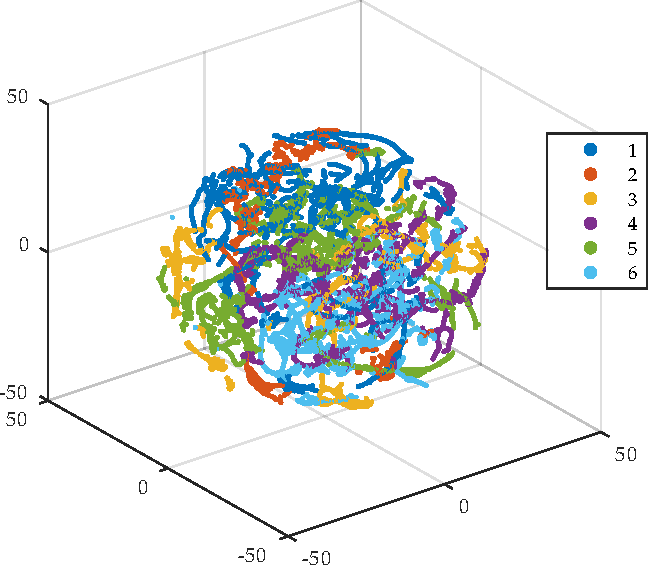
\includegraphics[width=\textwidth]{gfx/Chapter04/tsne_dsift_3d.pdf}
\caption{Distribution of the BOVW data of the RSM dataset in a reduced 3D space when visualised with t-SNE. Colours refer to different corridors in the dataset. Note that there is some evidence of the locally connected paths in the visual-words space.}
\label{fig:tsne3d}
\end{figure}

In Figure \ref{fig:tsne3d} we can see the 4,000-dimension visual word reduced to three dimensions and in Figure \ref{fig:tsne2d} we can see the two-dimensional embedding. The embeddings were generated using more than 50,000 randomly selected examples from all the corridors. Following the method described in Section~\ref{sec:quant_and_encod}, I selected for this particular example dense-SIFT descriptors encoded with hard assignment (HA), using $k$-means to create the visual word examples.

As we can see from the images, the difficulty of generating two or three-dimensional embeddings of such a high dimensional and complex dataset is notable. However, there are patterns showing how examples from the same corridors can display a sequential relationship within the embeddings.


\begin{figure}
\centering
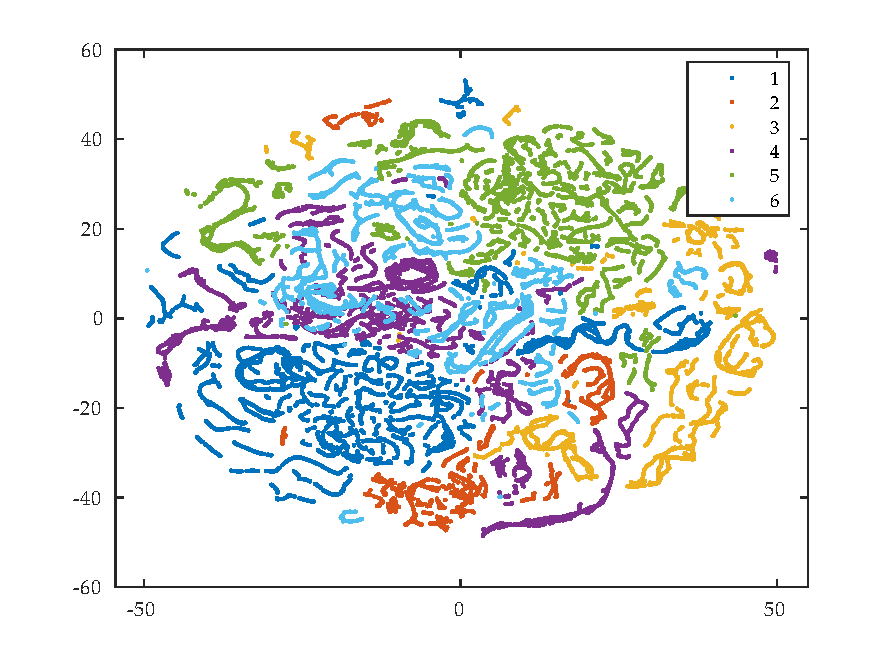
\includegraphics[width=\textwidth]{gfx/Chapter04/tsne_dsift_2d.pdf}
\caption{Distribution of the BOW data of the RSM dataset in a reduced 2D space when visualised with t-SNE. It is easy to identify some sets of points that form locally one-dimensional structures. Though they are not always contiguous for one corridor, the concept of visual paths appears at least partially justified.}
\label{fig:tsne2d}
\end{figure}

The present thesis gives an emphasis on understanding \textit{visual path} data from a journey perspective, from a crowdsourced collection of journeys in particular. However, although of limited practical use within journey localisation, this visualisation is the first step in understanding the structure of the data from a ``building'' perspective.

It is therefore subject of future work the use of these visualisations to understand the important features of visual paths datasets such as the presence of global clusters that reveal remarkable distinctiveness between journeys or give insight on how to optimise the retrieval based on between-journey differences.



%------------------------------------------------------------------------- 
\newpage
\section{Tactile feedback experiment protocol}
\subsection{Context}
The ``Visual localization with tactile feedback'' project aims to evaluate the quality of the tactile feedback given by the Senseg tablet in an indoor localization for the visually impaired context. When navigating a physical path, the user receives a tactile cue that encodes an estimate of their position along that specific path, relative to start and end point. Given several location estimate feedback cues through the Senseg tactile interface, the goal of this experiment is to evaluate how accurate this tactile feedback is based on the user perception of the position they are.

\subsection{Experiment protocol}

\begin{enumerate}

\item The user will be given some familiarization tasks with the Senseg demo that shipped with the tablet as Android applications. These will be:

\begin{itemize}
\item Familiarize with the different textures with the app ``Haptic Guidelines''.
\end{itemize}

\item The user will be given the following instructions:

\begin{framed}
You have agreed to take part in the ``Visual localization with tactile feedback" project experiment on tactile feedback quality. The experiment consists of the following tasks:

\begin{enumerate}
\item You will be given the Senseg tablet you used previously to get familiar with its tactile interface.

\item If you visually inspect the path, you will notice 2 red rectangles that denote starting and end point. These are texture highlighted. As you feel the screen with your finger and move it over the path you will notice four haptic ``landmarks'' or ``events'' that can be differentiated: 

\begin{enumerate}
\item the beginning of the path,
\item an area with no haptic feedback, this is the area that would represent the area that users have already traversed,
\item an area with haptic feedback, that represents the remaining segment of the path,
\item the end of the path, with highlighted haptic texture as event (i).
\end{enumerate}
\item You will receive one tactile cue every 15 seconds, making up to 20 cues. 

\item Upon the reception of the cue, it will be your task to announce an estimate of your location as a percentage of the total distance. You will only provide estimates that are 10\% apart:
\begin{itemize}
\item 0\%: starting point of the journey,
\item 10\%
\item 20\%,
\item ...
\item 80\%,
\item 90\%
\item 100\%: end point of the journey.
 
\end{itemize}

\item As agreed, you will blindfold yourself for this experiment. Please, proceed to wear the blindfold now, the experiment will start shortly.
\end{enumerate}
\end{framed}

\item The experiment will start:
\begin{enumerate}
\item The user will receive 20 tactile cues corresponding to 20 randomized location estimates provided by the localization server.
\item The users' announced estimates will be annotated next to their corresponding index in the following table\footnote{Not present in the volunteer copy.}


\begin{table}[h]
\centering
    \begin{tabular}{|c|c|c|}
    \hline Trial index & True location & Estimated location  \\ \hline
    1           & ~       0.81        	  &    \\ \hline
    2           & ~       0.91             &    \\ \hline
    3           & ~       0.13             &    \\ \hline
    4           & ~       0.91             &    \\ \hline
    5           & ~       0.63             &    \\ \hline
    6           & ~       0.10             &    \\ \hline
    7           & ~       0.28             &    \\ \hline
    8           & ~       0.55             &    \\ \hline
    9           & ~       0.96             &    \\ \hline
    10          & ~       0.16             &    \\ \hline
    11          & ~       0.49             &    \\ \hline
    12          & ~       0.80             &    \\ \hline
    13          & ~       0.14             &    \\ \hline
    14          & ~       0.42             &    \\ \hline
    15          & ~       0.79             &    \\ \hline
    16          & ~       0.66             &    \\ \hline
    17          & ~       0.04             &    \\ \hline
    18          & ~       0.93             &    \\ \hline
    19          & ~       0.40             &    \\ \hline
    20          & ~       0.27             &    \\ \hline
    \end{tabular}
\end{table}

\end{enumerate} 

\end{enumerate}

\newpage

\subsection{Informed consent form}

\subsubsection{Experiment purpose \& procedure}

The purpose of this experiment is to evaluate the quality of the tactile feedback given by the Senseg tablet in an indoor localization for the visually impaired context.

The experiment consists of 2 parts as detailed in the previous section

After the experiment, you will be asked to complete a feedback form.

Please note that none of the tasks is a test of your personal intelligence or ability. The objective is to test the usability of our research systems

\subsubsection{Confidentiality}

The following data will be recorded: Estimates of the tactile-encoded position along a path based on Senseg haptic feedback.

All data will be coded so that your anonymity will be protected in any research papers and presentations that result from this work.

\subsubsection{Finding out about result}

If interested, you can find out the result of the study by contacting the researcher Jose Rivera-Rubio, after 1 April 2015. 

His email address is jose.rivera@imperial.ac.uk.

\subsubsection{Record of consent}
Your signature below indicates that you have understood the information about the ``Tactile feedback with Senseg'' experiment and consent to your participation. The participation is voluntary and you may refuse to answer certain questions on the questionnaire and withdraw from the study at any time with no penalty. This does not waive your legal rights. You should have received a copy of the consent form for your own record. If you have further questions related to this research, please contact the researcher.


\def\info#1\par{#1\hrulefill\hss\par}
\everypar={\setbox0=\lastbox}
\baselineskip=15pt
\hsize=.5\hsize
\info Your Name

\info Your Signature

\vspace{1cm}

Researcher: Jose Rivera-Rubio


Date: 10/03/2015


\newpage